\newpage
\section{Implementacja}		%4
%Opisać implementacje algorytmu/programu. Pokazać ciekawe fragmenty kodu
%Opisać powstałe wyniki (algorytmu/nrzędzia)
\subsection{Struktura programu}
Program, jest narzędziem do zarządzania danymi w strukturze drzewa, które może być ładowane, analizowane, przetwarzane i zapisywane w różnych formatach. Służy do analizy danych związanych z różnymi parametrami (takimi jak autokonsumpcja, eksport, import, produkcja), przechowywanych w plikach CSV i plikach binarnych. Aplikacja pozwala użytkownikowi na wykonywanie różnych operacji na tych danych, takich jak obliczenia, wyszukiwanie, porównywanie oraz zapisywanie wyników w formie plików. Pliki które odpowiadają za działanie programu:
\\ \\
\textbf{Plik app.cpp}
\\
Odpowiada za interakcję z użytkownikiem i wywoływanie odpowiednich funkcji. Użytkownik wybiera opcje z menu, a aplikacja odpowiada na te wybory, wykonując odpowiednie operacje na danych (np. ładowanie danych, obliczenia).
\\ \\
\textbf{Plik lineData.cpp}
\\
Plik ten implementuje funkcje zadeklarowane w nagłówku lineData.hpp. Główne funkcje to konstrukcja obiektów LineData z danych wejściowych (zarówno z pliku tekstowego, jak i z pliku binarnego) oraz operacje na tych obiektach.
\\ \\
\textbf{Plik logger.cpp}
\\
Plik ten zawiera klasę Logger, która jest odpowiedzialna za rejestrowanie logów działania programu (zarówno informacji ogólnych, jak i błędów). Zawiera dwie instancje loggera: logger (do logów ogólnych) oraz loggerError (do logów błędów).
\\ \\
\textbf{Plik treeData.cpp}
\\
Plik ten zawiera klasę TreeData, która jest odpowiedzialna za zarządzanie strukturą danych w postaci drzewa. Drzewo to składa się z lat, miesięcy, dni i kwartałów, a każdy kwartał zawiera dane związane z pojedynczymi liniami danych. Plik treeData.cpp implementuje funkcje, które umożliwiają dodawanie danych, drukowanie ich, obliczanie sum, średnich, porównywanie danych pomiędzy okresami i inne operacje.
\\
\newpage
\subsection{Rozłożenie metody LineData::serialize(ofstream\& out) const}
Metoda jest odpowiedzialna za zapisanie wszystkich danych obiektu LineData do pliku w formacie binarnym, w tym rozmiaru i zawartości daty oraz wartości zmiennoprzecinkowych (autokonsumpcji, eksportu, importu, poboru i produkcji), co umożliwia efektywne przechowywanie i późniejsze odczytywanie tych danych. Metoda została przedstawiona na Listingu nr. \ref{lst:listing-cpp1} (s. \pageref{lst:listing-cpp1}): \\
\begin{lstlisting}[caption=LineData::serialize(ofstream\& out) const, label={lst:listing-cpp1}, language=C++]
void LineData::serialize(ofstream& out) const {
    size_t dateSize = date.size();
    out.write(reinterpret_cast<const char*>(&dateSize), sizeof(dateSize));
    out.write(date.c_str(), dateSize);
    out.write(reinterpret_cast<const char*>(&autokonsumpcja), sizeof(autokonsumpcja));
    out.write(reinterpret_cast<const char*>(&eksport), sizeof(eksport));
    out.write(reinterpret_cast<const char*>(&import), sizeof(import));
    out.write(reinterpret_cast<const char*>(&pobor), sizeof(pobor));
    out.write(reinterpret_cast<const char*>(&produkcja), sizeof(produkcja));
}
\end{lstlisting}
\textbf{Opis metody przedstawionej na listingu nr. \ref{lst:listing-cpp1} (s. \pageref{lst:listing-cpp1}):}
\begin{itemize}
    \item Kod oblicza długość ciągu date (czyli liczbę znaków w dacie) i zapisuje tę długość do pliku binarnego. Zmienna dateSize jest typu size\_t i przechowuje liczbę znaków w zmiennej date. Funkcja out.write() zapisuje tę liczbę jako ciąg bajtów do pliku. (Linia 2,3)
    \item Wiersze kodu zapisują zmienne zmiennoprzecinkowe do pliku binarnego. Zmienna jest przekonwertowana na wskaźnik, aby można było zapisać jej zawartość jako ciąg bajtów w formacie binarnym. Każda zmienna jest zapisywana z użyciem sizeof(), co zapewnia, że odpowiednia ilość bajtów jest zapisywana do pliku. (Linia 4-9)
\end{itemize}
\newpage
\subsection{Rozłożenie metody Logger::Logger(const std::string\& filename)}
Metoda ta jest odpowiedzialna za inicjalizację obiektu klasy Logger, tworzenie pliku logu z nazwą zawierającą datę i czas oraz otwieranie tego pliku do zapisu. Jeżeli plik o nazwie wynikowej już istnieje, zostaje usunięty przed otwarciem nowego pliku. Jeśli nie uda się otworzyć pliku, metoda zgłasza wyjątek. Metoda ta została przedstawiona na Listingu nr. \ref{lst:listing-cpp3} (s. \pageref{lst:listing-cpp3})
\begin{lstlisting}[caption=Logger::Logger(const std::string\& filename), label={lst:listing-cpp3}, language=C++]
Logger::Logger(const std::string& filename) {
    auto t = std::time(nullptr);
    std::tm tm;
    localtime_s(&tm, &t);
    std::ostringstream oss;
    oss << filename << "_" << std::put_time(&tm, "%d%m%Y_%H%M%S") << ".txt";
    std::string datedFilename = oss.str();
    if (std::remove(datedFilename.c_str()) != 0) {
    }
    logFile.open(datedFilename, std::ios::out | std::ios::app);
    if (!logFile.is_open()) {
        throw std::runtime_error("Nie mozna otworzyc logow");
    }
}
\end{lstlisting}
\textbf{Opis metody przedstawionej na Listingu nr. \ref{lst:listing-cpp3} (s. \pageref{lst:listing-cpp3}) }
\begin{itemize}
    \item W pierwszym kroku metoda uzyskuje aktualny czas systemowy, a następnie zamienia ten czas na strukturę tm reprezentującą lokalny czas. (Linia 2-4)
    \item Używając klasy std::ostringstream, generowana jest nazwa pliku, która składa się z podstawowej nazwy (przekazanej jako parametr filename), a następnie dodawany jest ciąg daty i czasu. Cała ta nazwa jest następnie konwertowana na ciąg znaków, który będzie używany do utworzenia pliku logu. (Linia 5-7)
    \item Przed otwarciem nowego pliku, metoda sprawdza, czy plik o wygenerowanej nazwie już istnieje. Jeśli tak, jest on usuwany. (Linia 8,9)
    \item Następnie, plik logu jest otwierany w trybie dopisania i zapisu. Jeśli otwarcie pliku się nie powiedzie, rzucany jest wyjątek z odpowiednią wiadomością błędu. (Linia 10-12)
\end{itemize}
\newpage
\subsection{Rozłożenie metody TreeData::addData(const LineData\& lineData)}
Metoda ta jest odpowiedzialna za dodanie nowych danych (obiekt LineData) do odpowiedniej struktury danych w drzewie (struktura years), przechowując dane zorganizowane według roku, miesiąca, dnia i kwartału. Na podstawie daty zawartej w obiekcie lineData metoda dzieli datę na poszczególne elementy (rok, miesiąc, dzień, godzina, minuta) i przypisuje dane do odpowiednich węzłów drzewa. Metoda ta została przedstawiona na Listingu nr. \ref{lst:listing-cpp2} (s. \pageref{lst:listing-cpp2}) \\
\begin{lstlisting}[caption=Metoda double oblicz\_pi, label={lst:listing-cpp2}, language=C++]
void TreeData::addData(const LineData& lineData) {
    stringstream ss(lineData.getDate());
    string token;
    vector<int> dateParts;

    while (getline(ss, token, '.')) {
        dateParts.push_back(stoi(token));
    }

    int year = dateParts[2];
    int month = dateParts[1];
    int day = dateParts[0];
    int hour = stoi(lineData.getDate().substr(11, 2));
    int minute = stoi(lineData.getDate().substr(14, 2));
    int quarter = (hour * 60 + minute) / 360;

    years[year].year = year;
    years[year].months[month].month = month;
    years[year].months[month].days[day].day = day;
    years[year].months[month].days[day].quarters[quarter].quarter = quarter;
    years[year].months[month].days[day].quarters[quarter].hour = hour;
    years[year].months[month].days[day].quarters[quarter].minute = minute;
    years[year].months[month].days[day].quarters[quarter].data.push_back(lineData);
}
\end{lstlisting}
\newpage 
\noindent\textbf{Opis metody przedstawionej na Listingu nr. \ref{lst:listing-cpp2} (s. \pageref{lst:listing-cpp2})}
\begin{itemize}
    \item Kod rozpoczyna od przetworzenia daty zawartej w obiekcie lineData. Metoda getDate() zwraca datę w formacie dd.mm.yyyy HH:MM. Następnie, za pomocą stringstream i funkcji getline(), data jest rozdzielana na poszczególne składniki: dzień, miesiąc i rok, które są następnie zapisane w dateParts. (Linia 2-8)
    \item Na podstawie rozdzielonej daty, wyciągane są poszczególne elementy: rok, miesiąc, dzień, godzina i minuta. Następnie, godzina i minuta są używane do obliczenia kwartału, przy czym kwartały są ustalane na podstawie czasu (np. pierwszy kwartał to godziny 00:00–00:59). (Linia 10-15)
    \item Na podstawie wyodrębnionych danych (rok, miesiąc, dzień, godzina, minuta, kwartał), metoda wstawia nowy obiekt lineData do odpowiedniego węzła w drzewie. Węzeł drzewa jest hierarchicznie zorganizowany, zaczynając od roku, przez miesiąc, dzień, kwartał, a na końcu dodawana jest sama data (lineData) do listy data w odpowiednim kwartale. (Linia 17-24)
\end{itemize}
\subsection{Działanie programu}
Program posiada interaktywne menu w którym użytkownik może wybrać jedną z opcji do wykonania. Menu zostało przedstawione na rysunku nr. \ref{rys:rysunek1} (s. \pageref{rys:rysunek1}) 
\begin{figure}[h]
    \centering
    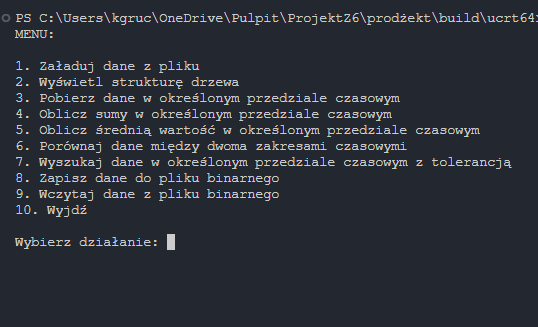
\includegraphics[width=0.8\linewidth]{img/1.png}
    \caption{Menu programu}
    \label{rys:rysunek1}
\end{figure}
\newpage
\noindent Teraz za pomocą 1 opcji użytkownik może wczytać do programu dane z pliku .csv, które można później poddać analizie, zostało to pokazane na rysunku nr. \ref{rys:rysunek2} (s. \pageref{rys:rysunek2}).
\\
\begin{figure}[h]
    \centering
    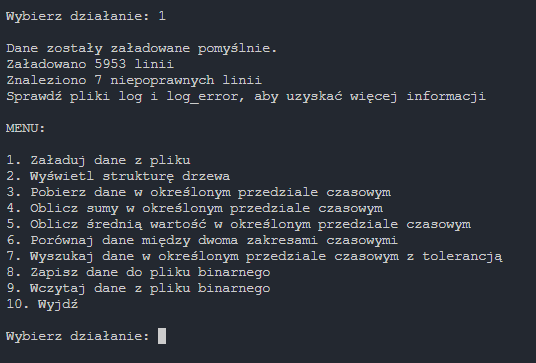
\includegraphics[width=0.8\linewidth]{img/2.png}
    \caption{Załadowanie pliku .csv}
    \label{rys:rysunek2}
\end{figure} \\
Jak widzimy na rysunku nr. \ref{rys:rysunek2} (s. \pageref{rys:rysunek2}) z pliku .csv zostało załadowane poprawnie 5953 linii, oraz znaleziono 7 niepoprawnych linii, aby uzyskać informacje na temat tego błędu, użytkownik może zobaczyć pliki z logami, które program generuje. Teraz możemy przejść do testu np. 3 opcji, wybieramy ją i wpisujemy ramy czasowe tak jak na rysunku nr. \ref{rys:rysunek3} (s. \pageref{rys:rysunek3})
\begin{figure}[h]
    \centering
    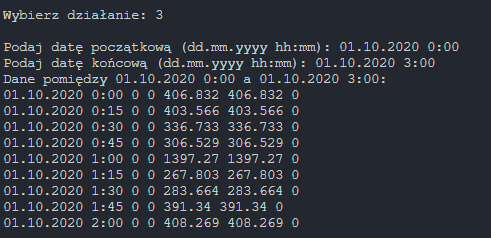
\includegraphics[width=0.8\linewidth]{img/4.png}
    \caption{Testowanie opcji}
    \label{rys:rysunek3}
\end{figure}
\newpage
\noindent Jak widzimy na rysunku nr. \ref{rys:rysunek3} (s. \pageref{rys:rysunek3}), dane zostały prawidłowo wypisane z pliku .csv zgodnie z wybranym przedziałem czasowym. Teraz możemy sobie zapisać nasze dane do plku binarnego, tak jak zostało to pokazane na rysunku nr.  \ref{rys:rysunek5} (s. \pageref{rys:rysunek5}).
\begin{figure}[h]
    \centering
    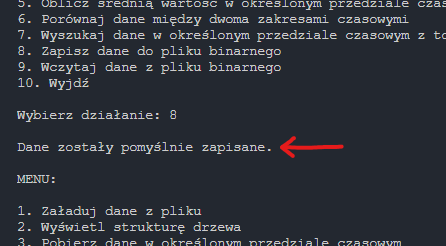
\includegraphics[width=0.8\linewidth]{img/5.png}
    \caption{Zapis do pliku binarnego}
    \label{rys:rysunek5}
\end{figure} \\
Możemy przetestować jeszcze 5 opcję która oblicza średnie wartości w określonym przedziale czasowym, działanie zostało przedstawione na rysunku nr. \ref{rys:rysunek6} (s. \pageref{rys:rysunek6}).
\begin{figure}[h]
    \centering
    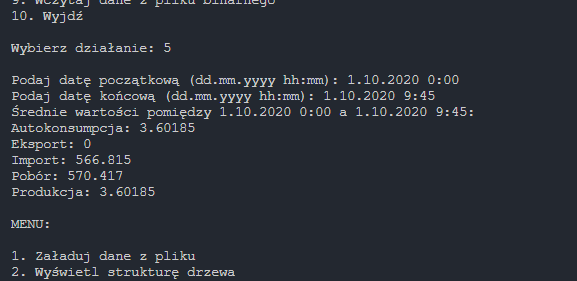
\includegraphics[width=0.8\linewidth]{img/6.png}
    \caption{Testowanie opcji programu}
    \label{rys:rysunek6}
\end{figure}
\newpage
\subsection{Testy programu}
W projekcie został przeprowadzony test za pomocą frameworka Google Test, który umożliwił dokładną weryfikację poprawności działania kluczowych modułów aplikacji. Na rysunku nr. \ref{rys:rysunek7} (s. \pageref{rys:rysunek7})  został przeprowadzony zrzut z wykonanych testów. 
\\ 
\begin{figure}[h]
    \centering
    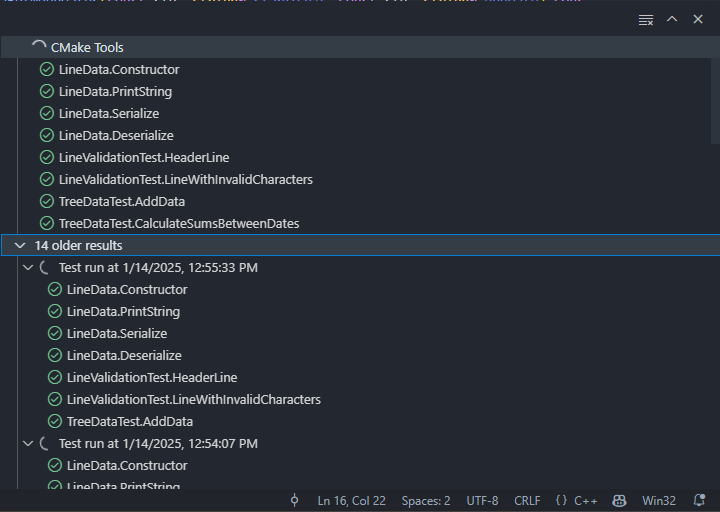
\includegraphics[width=0.8\linewidth]{img/test.png}
    \caption{Testy kodu za pomocą Google Test}
    \label{rys:rysunek7}
\end{figure} \\
\noindent Google Test został wybrany, ponieważ jest to narzędzie wydajne, elastyczne i dostosowane do wymagań projektu. Jego zastosowanie umożliwiło szybkie i dokładne przeprowadzenie testów jednostkowych, zwiększając niezawodność aplikacji. W projekcie do testowania można było jeszcze użyt takiego narzędzie jak Catch2 który jest bardzo łatwy w użyciu oraz ma intuicyjny system asercji i czytelne raport o wynikach testów, lecz jest mniej zaawansowany niż Google Test w przypadku bardziej złożonych scenariuszy, takich jak testy parametrów czy współpraca z dużymi projektami.
\newpage
\subsection{Pomoc AI w projekcie}
W projekcie został wykorzystany GitHub Copilot, który pomógł przy pisaniu różnych fragmentów kodu. AI szczególnie był pomocny przy:
\begin{itemize}
    \item \textbf{Generowanie szkieletu kodu} - Copilot był szczególnie pomocny w tworzeniu szkieletu kodu. Automatycznie proponował struktury funkcji, deklaracje klas oraz szablony kodu bazujące na nazwach funkcji i zmiennych. To znacznie przyspieszyło proces tworzenia początkowych wersji modułów, takich jak obsługa menu czy operacje na plikach.
    \item \textbf{Operacje na strukturach danych} - Podczas implementacji funkcji dla struktury drzewa (treeData.hpp), Copilot dobrze sugerował metody wyszukiwania, filtrowania i iteracji po węzłach. Przyspieszyło to implementację takich funkcji, jak obliczanie sum czy wyszukiwanie danych w przedziale czasowym.
    \item \textbf{Obsługa plików} - Przy implementacji funkcji wczytywania i zapisywania danych (CSV, binarne), Copilot pomógł w generowaniu kodu do operacji na plikach, takich jak otwieranie plików, odczytywanie danych w pętlach oraz zapisywanie ich w odpowiednich formatach. Umożliwiło to skrócenie czasu pracy nad tymi funkcjami.
\end{itemize}
Copilot nie był pomocny w kilku kwestiach:
\begin{itemize}
    \item \textbf{Specyficzne wymagania projektu} - Copilot często sugerował ogólne rozwiązania, które nie zawsze pasowały do wymagań projektu. Na przykład przy pracy z niestandardową strukturą drzewa (TreeData) lub specyficznym formatem danych w plikach CSV konieczne było ręczne dopracowywanie kodu. Podpowiedzi wymagały dostosowania do rzeczywistych potrzeb projektu.
    \item \textbf{Logika biznesowa i analizy danych} - Chociaż Copilot był pomocny w pisaniu szkieletu funkcji, nie zawsze trafnie rozumiał zaawansowane operacje, takie jak obliczanie średnich, porównywanie danych między zakresami czasowymi czy implementacja tolerancji w wyszukiwaniu. Te fragmenty wymagały manualnego dostosowania.
\end{itemize}
